\subsection*{Анализ показателей Японии}
\addcontentsline{toc}{subsection}{Анализ показателей Японии}

\textbf{Задание:}\\
Выбрать значимые показатели для рассмотрения динамики экономики страны, сделать прогнозы и описать полученные результаты по миграции данной страны в кластерах.\\

\textbf{Решение:}\\
В качестве рассматриваемой страны была выбрана Япония.\\

Были рассмотрены следующие показатели:
\begin{enumerate}[topsep=0pt,itemsep=-1ex,partopsep=1ex,parsep=1ex]
	\item численность людей (тыс.)
	\item численность молодого населения 0-14 (\% от общей численности)
	\item темпы роста ВВП (\%)
	\item уровень безработицы (\% от всей рабочей силы)
	\item уровень экспорта (\% от ВВП)
	\item уровень импорта (\% от ВВП)
	\item подушевой ВВП (текущих US\$)\\
\end{enumerate}

Эти данные были взяты с сайта Всемирного банка [9.10.2022]. (Рисунок \ref{fig:japan_data})

\begin{figure}[h]
	\centering 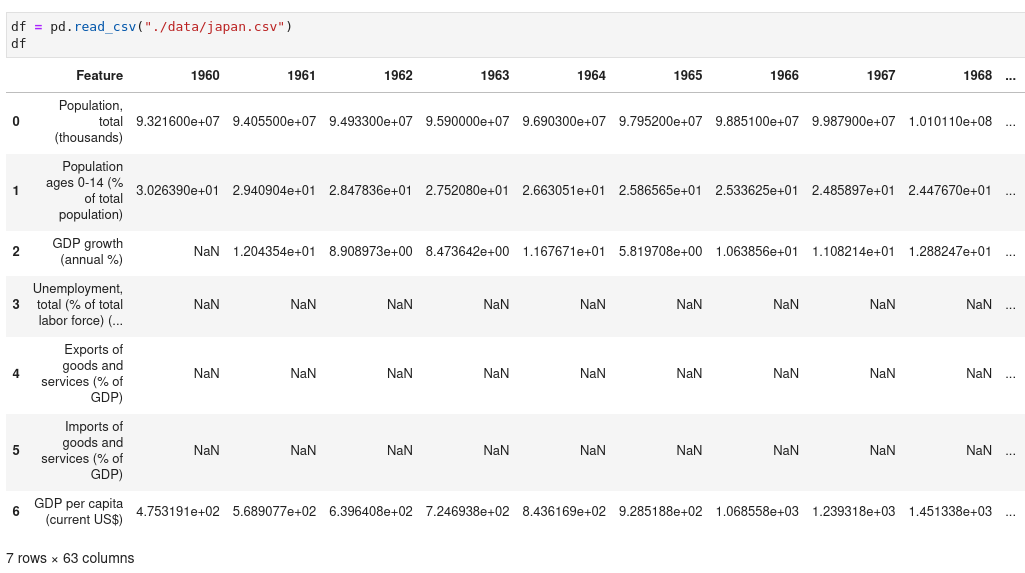
\includegraphics[scale=0.45]{japan_data}
	\caption{Выбранные показатели Японии с 1960 года по 2021 год}
	\label{fig:japan_data}
\end{figure}

\newpage

Далее был рассмотрен каждый показатель отдельно.\\
На основе данных можно построить график как менялась численность населения. (Рисунок \ref{fig:japan_population_plot})

\begin{figure}[h]
	\centering 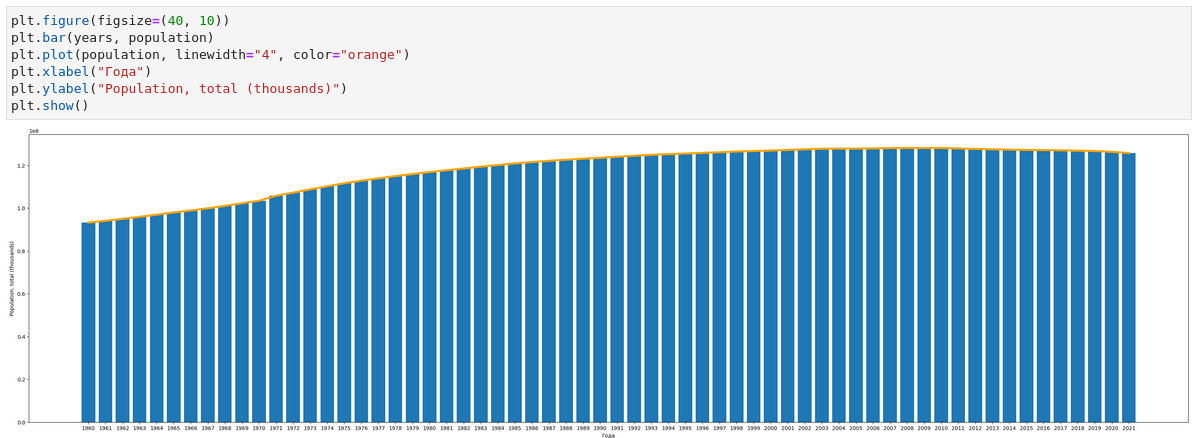
\includegraphics[scale=0.42]{japan_population_plot}
	\caption{Динамика численности населения Японии с 1960 года по 2021 год}
	\label{fig:japan_population_plot}
\end{figure}

Можно заметить, что до 2005-2006 года наблюдался рост численности людей, после уровень популяции вышел на плато, а затем (с 2010 года) начал постепенно убывать.\\

Стоит также проанализировать и <<молодую>> часть населения Японии. (Рисунок \ref{fig:japan_young_population_plot})

\begin{figure}[h]
	\centering 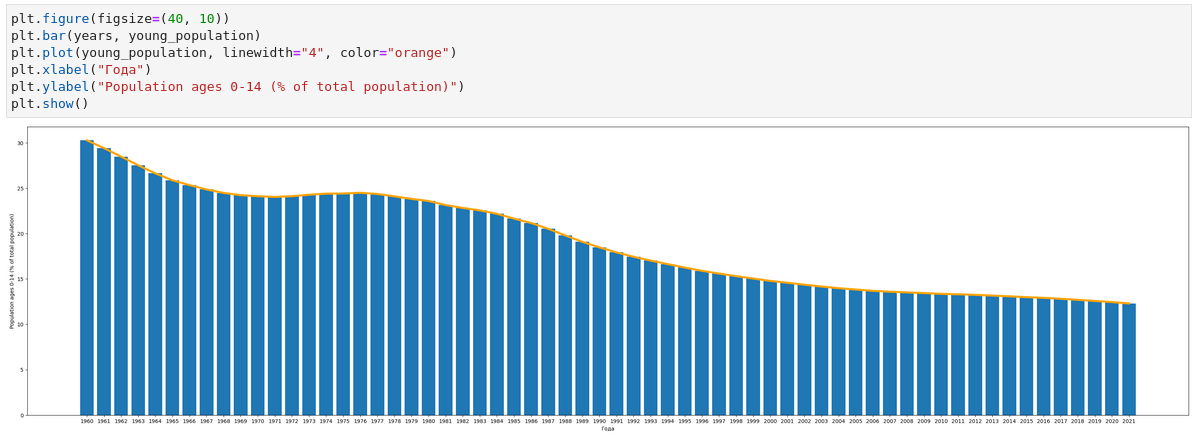
\includegraphics[scale=0.42]{japan_young_population_plot}
	\caption{Динамика молодого населения Японии с 1960 года по 2021 год}
	\label{fig:japan_young_population_plot}
\end{figure}

На графике видно, что детей становится с каждым годом всё меньше и меньше.

\newpage

Проблема демографии не обошла и Японию, по демографическим пирамидам можно заметить, что на сегодняшний день основную часть населения составляют люди в <<зрелом>> возрасте. Как можно заметить из возрастно-половых пирамид, если ничего не поменяется, то прогнозируют, что к 2050 году в Японии сократится население на 20 миллионов человек. (Рисунок \ref{fig:japan_pyramid})

\begin{figure}[h]
	\centering 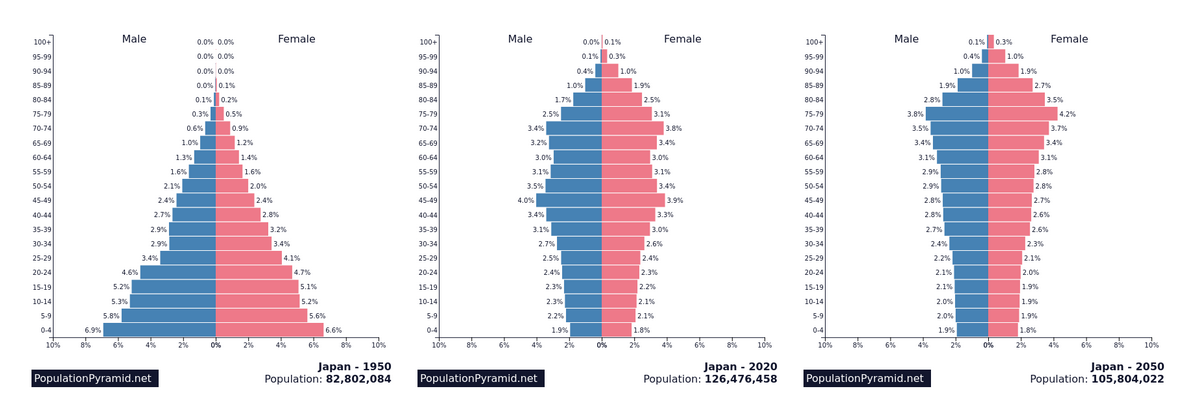
\includegraphics[scale=0.43]{japan_pyramid}
	\caption{Возрастно-половые пирамиды}
	\label{fig:japan_pyramid}
\end{figure}

Далее было рассмотрено изменение темпов роста ВВП. (Рисунок \ref{fig:japan_gdp_growth_plot})

\begin{figure}[h]
	\centering 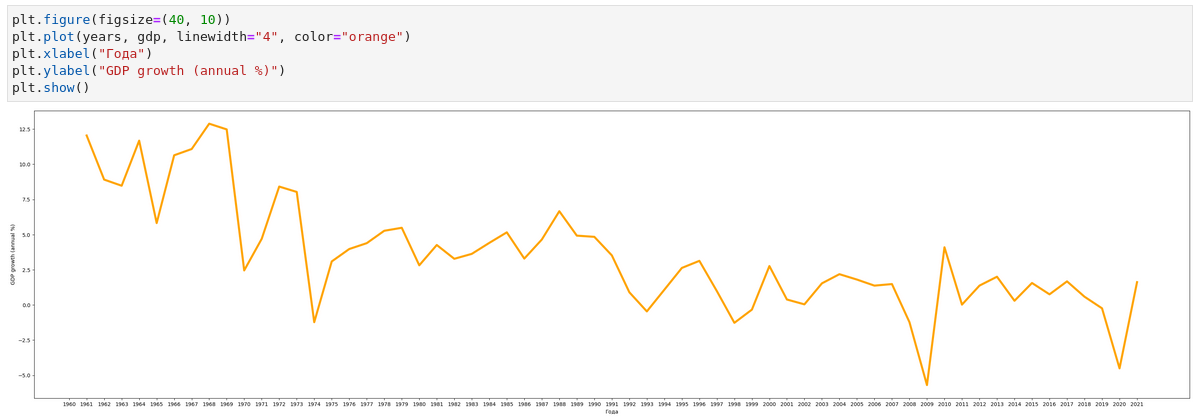
\includegraphics[scale=0.43]{japan_gdp_growth_plot}
	\caption{Динамика темпов роста ВВП Японии с 1960 года по 2021 год}
	\label{fig:japan_gdp_growth_plot}
\end{figure}

Можно заметить что с середины 1950 до 1973 года темпы прироста ВВП были достаточно велики, составляли более 10\% ежегодно и это были самые высокие показатели прироста ВВП среди развитых стран того времени. Этот феномен называют <<Японское экономическое чудо>>.

\newpage

Причины данного феномена:
\begin{itemize}[topsep=0pt,itemsep=-1ex,partopsep=1ex,parsep=1ex]
	\item дешевизна рабочей силы
	\item объединение производителей, поставщиков ресурсов, сбытчиков продукции и банков в тесно связанные группы
	\item взаимовыгодные отношения предпринимателей с правительством
	\item Корейская война, поставка вооружения США через Японию
	\item отсутствие военных расходов у Японии (отказ от милитаристского бюджета). В 1972 году его доля составила только 1\% от ВНП
	\item освоение японской наукой новых технологий, скупка патентов и лицензий
	\item \dots\\
\end{itemize}

Также можно заметить, что присутствуют спады, а именно в 1973 году случился Нефтяной кризис, а так как Япония в те годы делала упор на химическую промышленность, в том числе и переработку нефти, то на их экономики это тоже сказалось. Ещё имеются спады в 2008 году и 2020 году, в 2008 году произошёл Мировой кризис, а в 2020 году был COVID-19.\\

Если посмотреть, то за исключением кризисов был стабильный ежегодный прирост ВВП в среднем на 2.24\%, что достаточно хорошо.\\

Следующий фактор, который был проанализирован -- это динамика уровня безработицы. (Рисунок \ref{fig:japan_unemployment_plot})

\begin{figure}[h]
	\centering 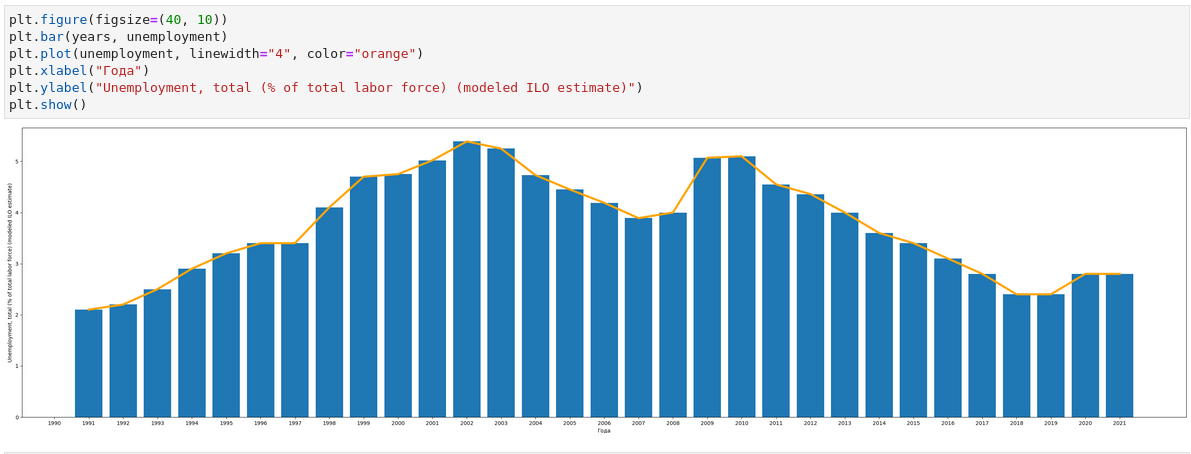
\includegraphics[scale=0.42]{japan_unemployment_plot}
	\caption{Динамика уровня безработицы Японии с 1991 года по 2021 год}
	\label{fig:japan_unemployment_plot}
\end{figure}

Можно заметить, что уровень безработицы в Японии достаточно низкий и в среднем составляет 3.7\%.

\newpage

Далее рассматривалась динамика объёмов экспорта. (Рисунок \ref{fig:japan_export_plot})

\begin{figure}[h]
	\centering 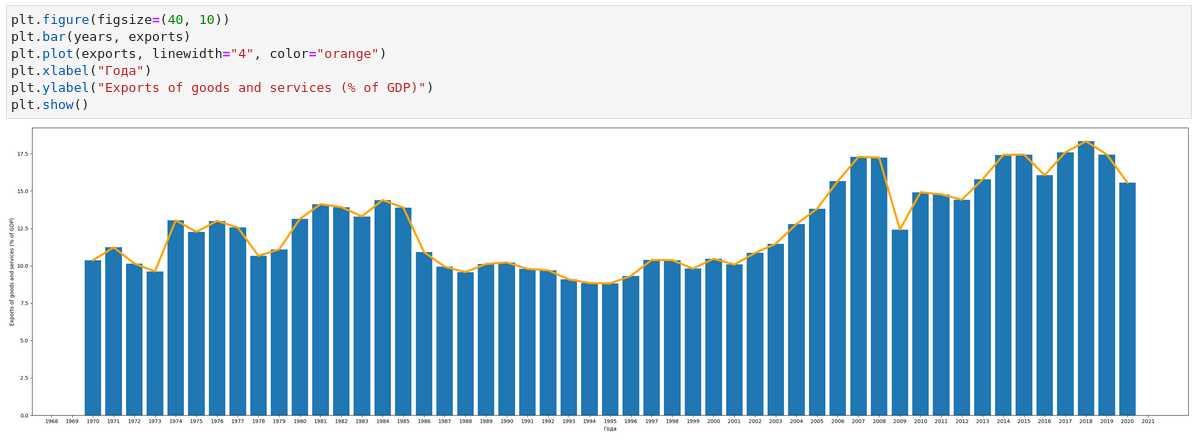
\includegraphics[scale=0.42]{japan_export_plot}
	\caption{Динамика объёмов экспорта Японии с 1970 года по 2020 год}
	\label{fig:japan_export_plot}
\end{figure}

Страна не очень богата природными ресурсами, но тем не менее она является одним из главных мировых экспортёров в отраслях:
\begin{itemize}[topsep=0pt,itemsep=-1ex,partopsep=1ex,parsep=1ex]
	\item робототехники
	\item автомобилестроения
	\item электронно-вычислительной техники
	\item бытовой химии\\
\end{itemize}

И также были рассмотрены изменения уровня объёма импорта. (Рисунок \ref{fig:japan_import_plot})

\begin{figure}[h]
	\centering 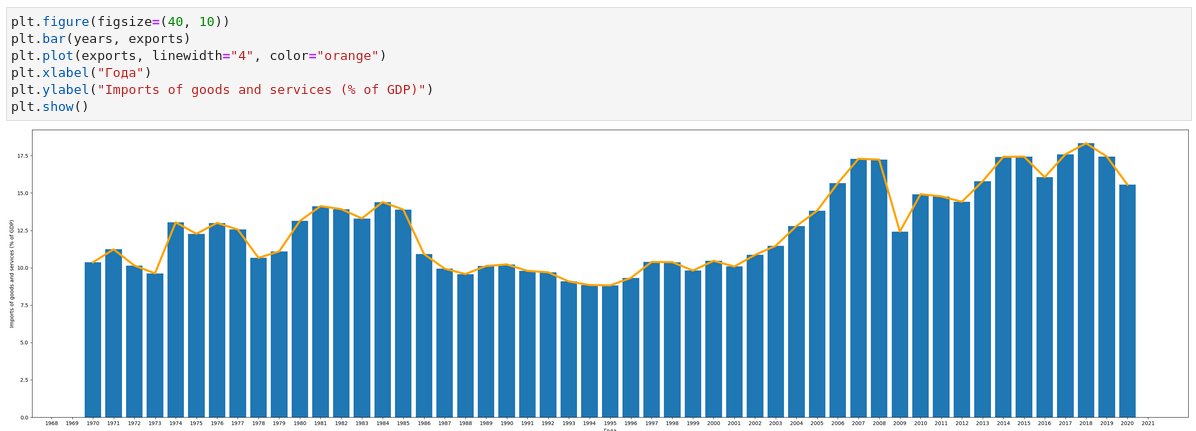
\includegraphics[scale=0.42]{japan_import_plot}
	\caption{Динамика объёмов импорта Японии с 1970 года по 2020 год}
	\label{fig:japan_import_plot}
\end{figure}

\newpage

Основными товарами импорта являются:
\begin{itemize}[topsep=0pt,itemsep=-1ex,partopsep=1ex,parsep=1ex]
	\item минеральные ресурсы
	\item текстильные товары
	\item металло-продукция
	\item продукты питания\\
\end{itemize}

Последний рассмотренный фактор -- это динамика подушевого ВВП. (Рисунок \ref{fig:japan_gdp_per_capita_plot})

\begin{figure}[h]
	\centering 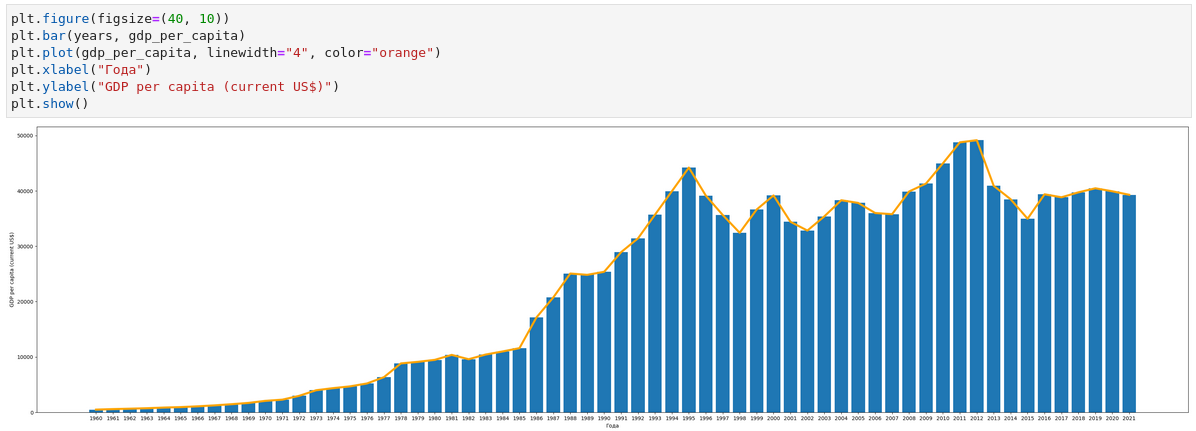
\includegraphics[scale=0.42]{japan_gdp_per_capita_plot}
	\caption{Динамика объёмов подушевого ВВП Японии с 1970 года по 2020 год}
	\label{fig:japan_gdp_per_capita_plot}
\end{figure}

Можно видеть, что когда Япония проиграла Вторую мировую войну, то страна была разрушена и ВВП был достаточно низок, а численность населения была большой. Однако потом страна начала наращивать темпы роста ВВП и произошло <<Японское экономическое чудо>>, после чего темпы подушевого ВВП выросли и сейчас достаточно стабильны.\\

Далее были построены прогнозы на 10 лет для каждого из признаков с помощью модели прогнозирования \textit{SARIMAX}. Для каждого признака были подобраны оптимальные значения $p$ и $q$ c помощью графиков автокорреляции и частичной автокорреляции.\\

\newpage

Первым было спрогнозировано изменение уровня безработицы. (Рисунок \ref{fig:japan_unemployment_plot_forecast})

\begin{figure}[h]
	\centering 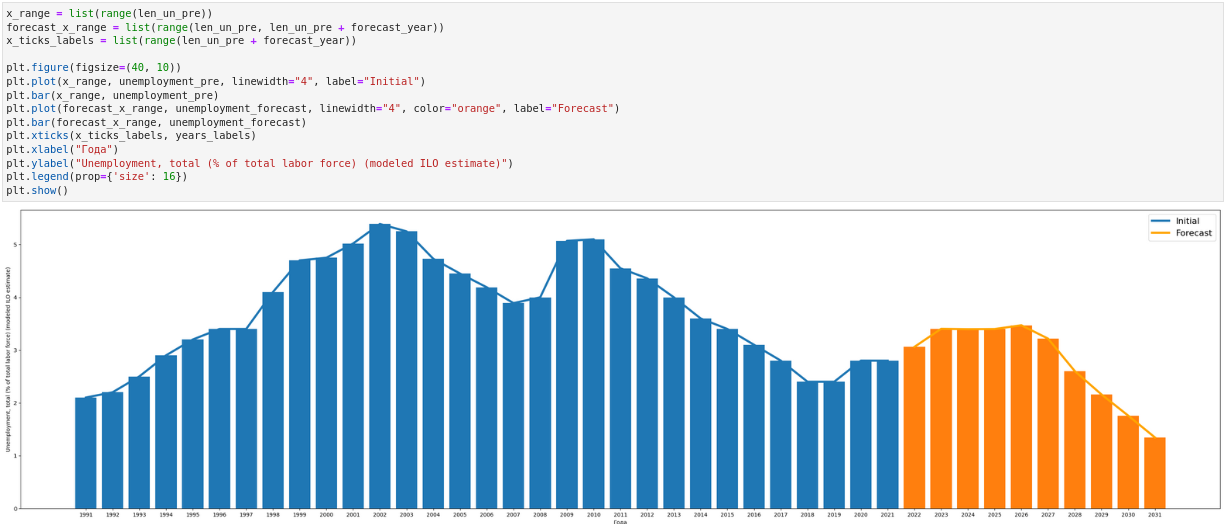
\includegraphics[scale=0.42]{japan_unemployment_plot_forecast}
	\caption{Прогноз динамики уровня безработицы Японии на 10 лет}
	\label{fig:japan_unemployment_plot_forecast}
\end{figure}

Можно видеть, что в ближайшие 10 лет будет ожидаться сначала стабильный уровень безработицы, а затем он будет уменьшаться.\\

Далее было решено спрогнозировать динамику темпов роста ВВП. (Рисунок \ref{fig:japan_gdp_growth_forecast})

\begin{figure}[h]
	\centering 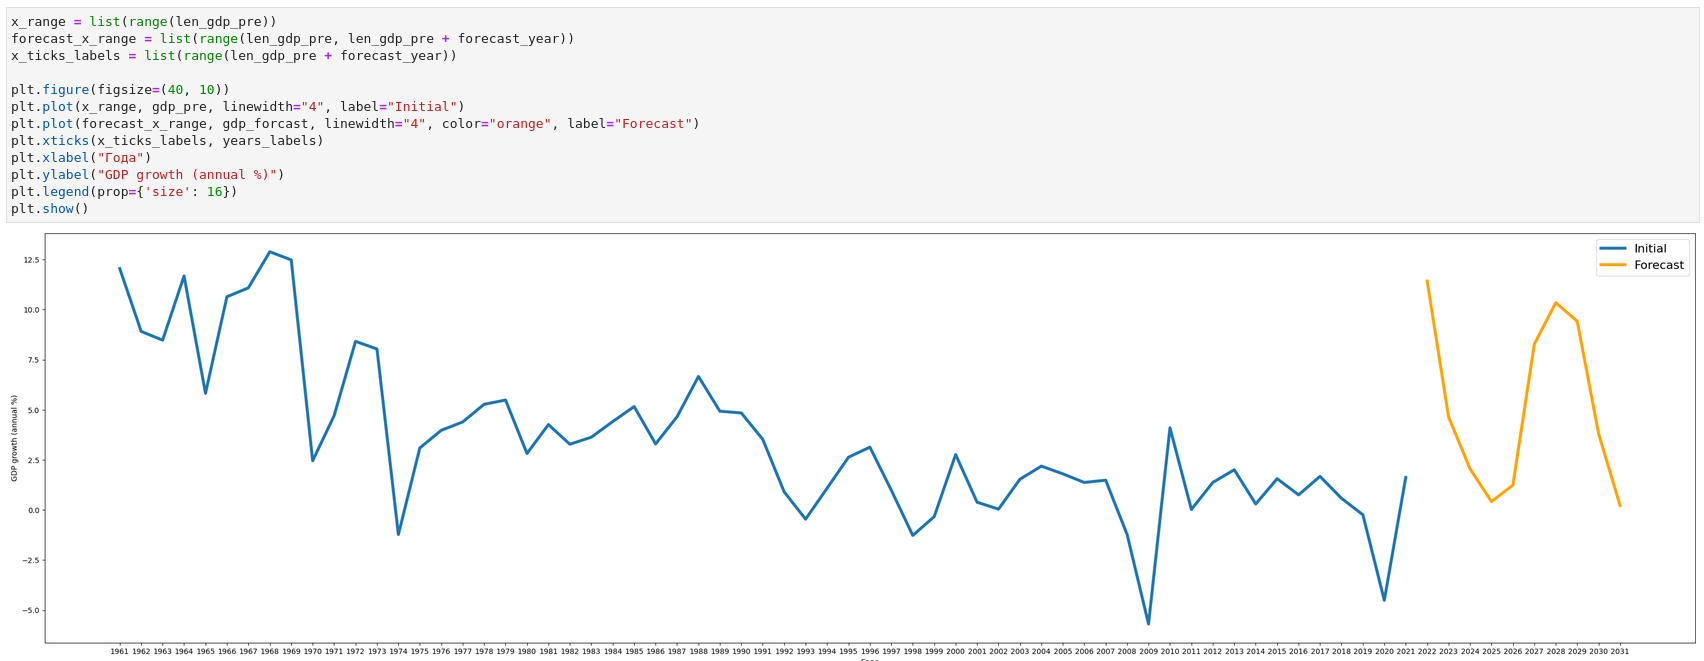
\includegraphics[scale=0.3]{japan_gdp_growth_forecast}
	\caption{Прогноз динамики темпов роста ВВП Японии на 10 лет}
	\label{fig:japan_gdp_growth_forecast}
\end{figure}

\newpage

На графике можно видеть, что ожидается рост темпов роста ВВП, а затем он снова должен нормализироваться.\\

Также было спрогнозировано изменение численности молодого населения в стране. (Рисунок \ref{fig:japan_young_population_forecast})

\begin{figure}[h]
	\centering 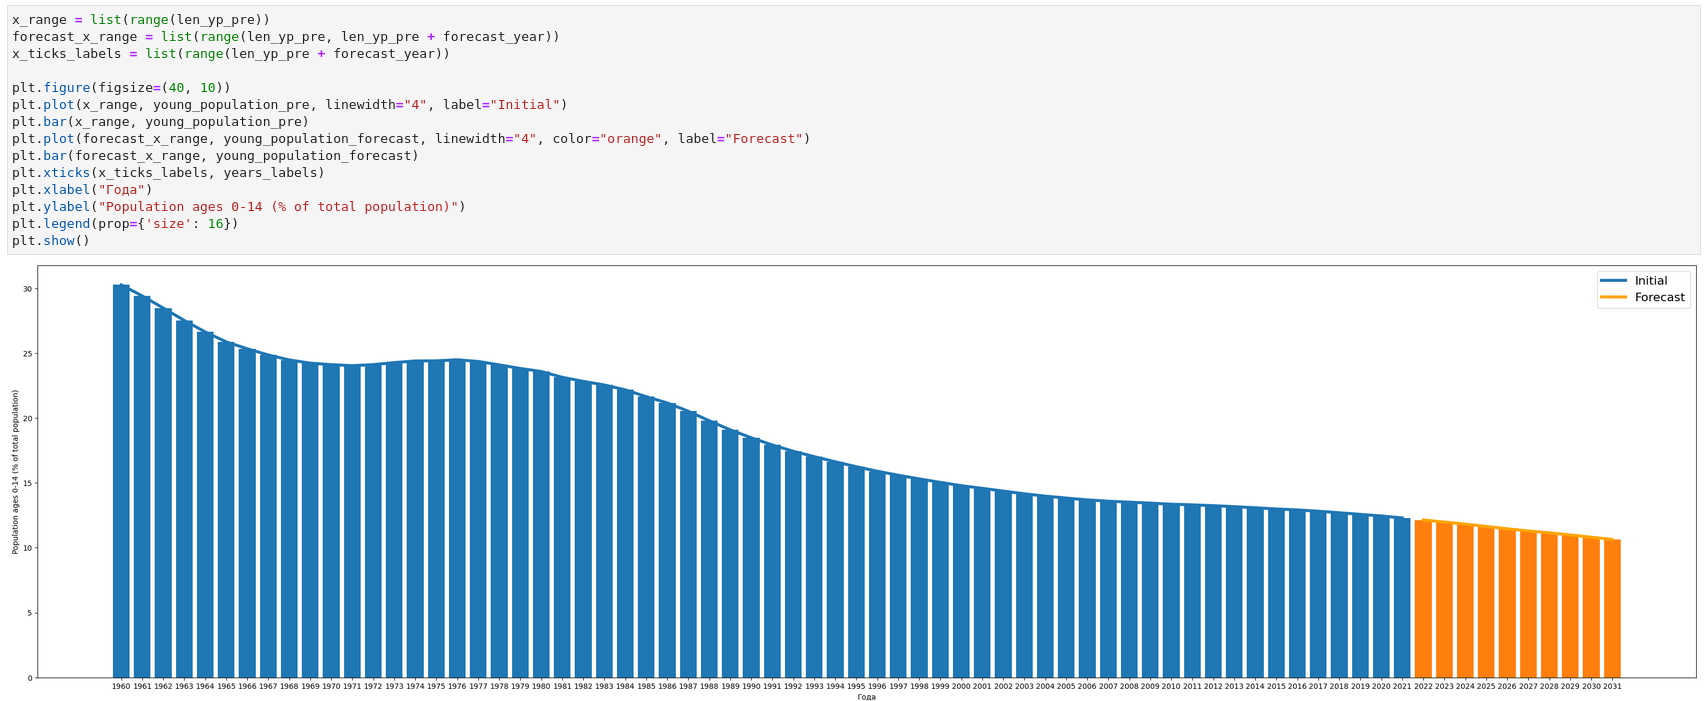
\includegraphics[scale=0.3]{japan_young_population_forecast}
	\caption{Прогноз изменения численности молодого населения Японии на 10 лет}
	\label{fig:japan_young_population_forecast}
\end{figure}

Как уже было ранее сказано, что если ничего не поменяется, то ожидается, что численность населения в Японии сократиться на 20 миллионов человек.\\

Последнее что было спрогнозировано -- это изменение уровня экспорта.  (Рисунок \ref{fig:japan_export_forecast})

\begin{figure}[h]
	\centering 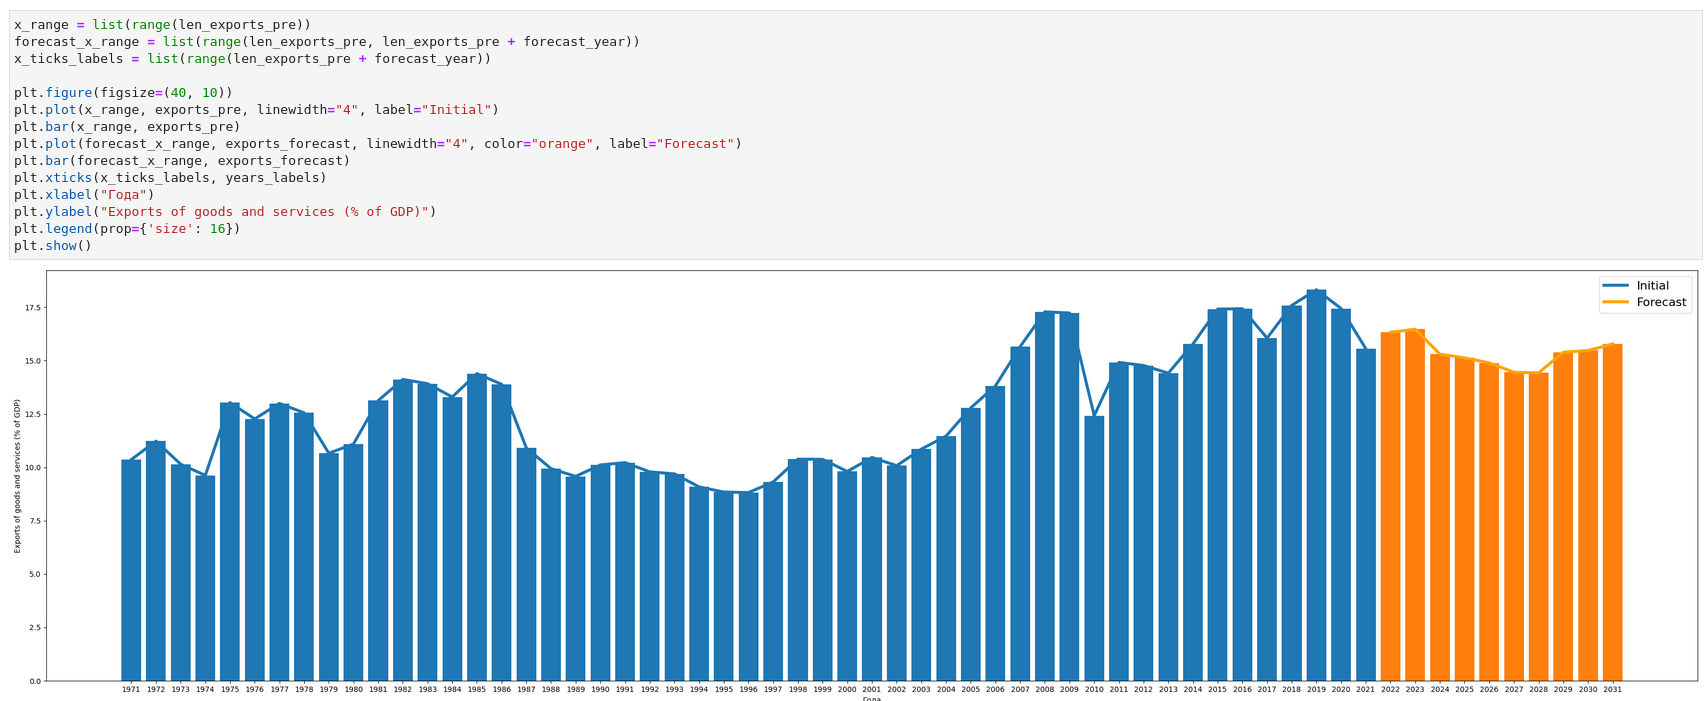
\includegraphics[scale=0.25]{japan_export_forecast}
	\caption{Прогноз изменения уровня экспорта Японии на 10 лет}
	\label{fig:japan_export_forecast}
\end{figure}

\newpage

На данном графике видно, что уровень экспорта останется примерно стабильным.\\

Также на основе построенных кластеров было выявлено, что в 2013 году Япония находилась в кластере стран со средним темпом роста подушевого ВВП, в 2019 году её кластер не изменился.\\

В 2013 году Япония находилась в кластере стран со средним темпом роста ВВП, в 2019 году она оказалась в кластере с низким темпом роста ВВП.\\

В 2013 году Япония находилась в кластере с низким темпом инфляции, в 2019 году её кластер не изменился.